\documentclass[
	fontsize=12pt,
	paper=a4,
	numbers=noenddot,
	listof=totoc,
	listof=entryprefix,
	listof=nochaptergap,
	bibliography=totoc,
	parskip=half,
	openany
]{scrbook}

\include{../../for_latex/preamble}

\begin{document}

\begin{titlepage}
	\pagestyle{empty}

	\begin{flushright}
		\begin{figure}[ht]
			\flushright
			
\includegraphics[height=2cm]{../../for_latex/hfu}
		\end{figure}
	\end{flushright}

	\begin{center}
		\vspace{3cm}

		{\fontsize{22}{22} \selectfont \textbf{Blatt 4}}\\[5mm]
		{\fontsize{18}{18} \selectfont Grundlagen der IT-Sicherheit}

		\vspace{12cm}

		{\fontsize{14}{14} \selectfont Luis Staudt}
	\end{center}
\end{titlepage}

% ############################################################################
% CONTENT STARTS HERE
% ############################################################################

\chapter*{Aufgabe 1: Signieren, verschlüsseln und entschlüsseln}

\section*{a) Schlüsselpaar erstellen}

Mit dem Befehl \texttt{gpg --gen-key} wurde ein Schlüsselpaar für die Adresse
\texttt{lst48606@stud.hs-furtwangen.de} erstellt.
Die Ausgabe von \texttt{gpg -k} zeigt beide vorhandenen öffentlichen Schlüssel:

\begin{figure}[H]
	\centering
	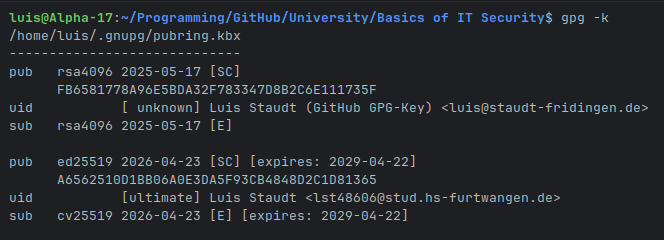
\includegraphics[width=\textwidth]{images/gpg_k_nach_keygen}
	\caption{Ausgabe von \texttt{gpg -k} nach der Schlüsselerstellung}
\end{figure}

Der neu erstellte Schlüssel hat den Fingerprint:\\
\texttt{A656 2510 D1BB 06A0 E3DA 5F93 CB48 48D2 C1D8 1365}

\section*{b) Öffentlichen Schlüssel exportieren}

Der öffentliche Schlüssel wurde mit folgendem Befehl im ASCII-Format exportiert:

\begin{lstlisting}[language=bash]
gpg --output Luis.Staudt.gpg --armor --export lst48606@stud.hs-furtwangen.de
\end{lstlisting}

Der Schalter \texttt{--armor} sorgt dafür, dass der Schlüssel als druckbarer ASCII-Text
ausgegeben wird, was die Übertragung per E-Mail oder andere Textmedien vereinfacht.
Die Datei \texttt{Luis.Staudt.gpg} wurde anschließend im Felix-Kurs hochgeladen.

\section*{c) Datei erstellen und signieren}

Es wurde eine Textdatei \texttt{LuisStaudt.txt} mit dem Inhalt
\textit{\glqq Ich überweise 50 Euro\grqq{}} erstellt und anschließend signiert:

\begin{lstlisting}[language=bash]
gpg --detach-sign -u lst48606@stud.hs-furtwangen.de LuisStaudt.txt
\end{lstlisting}

Dabei entsteht die Datei \texttt{LuisStaudt.txt.sig}, die die digitale Signatur enthält.
Beide Dateien wurden im Felix-Kurs hochgeladen.

\section*{d) Signatur einer anderen Datei prüfen (vor Key-Import)}

Mit folgendem Befehl wurde die Signatur der Datei von Ben Barfuss geprüft:

\begin{lstlisting}[language=bash]
gpg --verify Ben.Barfuss.txt.sig Ben.Barfuss.txt
\end{lstlisting}

\begin{figure}[H]
	\centering
	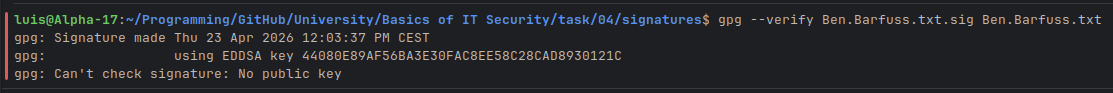
\includegraphics[width=\textwidth]{images/signaturpruefung_vor_import}
	\caption{Signaturprüfung vor dem Import des öffentlichen Schlüssels}
\end{figure}

GPG meldet \textit{Can't check signature: No public key}, da der öffentliche Schlüssel
von Ben Barfuss noch nicht im lokalen Schlüsselbund vorhanden ist.

Die Prüfung hat zu diesem Zeitpunkt noch keine Bedeutung, da ohne den öffentlichen
Schlüssel des Absenders gar keine Überprüfung möglich ist.
Selbst wenn der Schlüssel vorliegen würde, wäre nicht sichergestellt, dass er
tatsächlich der angegebenen Person gehört, da noch kein Vertrauen (Trust) etabliert wurde.

\section*{e) Öffentliche Schlüssel importieren}

Der öffentliche Schlüssel wurde mit folgendem Befehl importiert:

\begin{lstlisting}[language=bash]
gpg --import Ben.Barfuss.gpg
\end{lstlisting}

Nach dem Import wurde die Signatur erneut geprüft:

\begin{figure}[H]
	\centering
	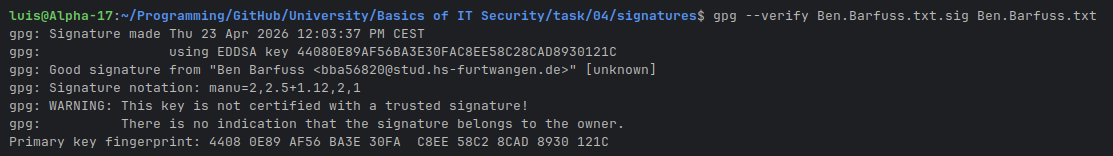
\includegraphics[width=\textwidth]{images/signaturpruefung_nach_import}
	\caption{Signaturprüfung nach dem Import des öffentlichen Schlüssels}
\end{figure}

GPG meldet nun \textit{Good signature from \glqq Ben Barfuss\grqq{}}, fügt jedoch hinzu:
\textit{This key is not certified with a trusted signature!}
Die Prüfung funktioniert technisch, aber der Schlüssel gilt als \texttt{[unknown]}.

Es kann nicht sichergestellt werden, dass der importierte Schlüssel wirklich zu Ben Barfuss gehört,
da er lediglich aus dem Felix-Kurs heruntergeladen wurde, ohne die Identität des Besitzers
persönlich verifiziert zu haben.
Ein Angreifer könnte einen gefälschten Schlüssel unter dem Namen eines Kommilitonen hochgeladen haben.

\section*{f) Erhaltenen Schlüssel signieren}

Der Fingerprint des importierten Schlüssels wurde persönlich mit dem Kommilitonen abgeglichen.
Anschließend wurde der Schlüssel mit folgendem Befehl signiert:

\begin{lstlisting}[language=bash]
gpg --edit-key bba56820@stud.hs-furtwangen.de
gpg> trust    # trust level: full
gpg> tsign    # trust depth: 2, no domain restriction
gpg> save
\end{lstlisting}

\begin{figure}[H]
	\centering
	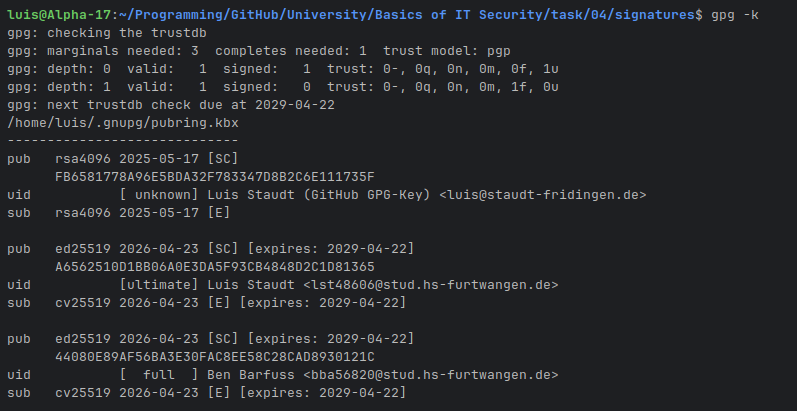
\includegraphics[width=\textwidth]{images/gpg_k_nach_signieren}
	\caption{Ausgabe von \texttt{gpg -k} nach dem Signieren des Schlüssels}
\end{figure}

Ben Barfuss' Schlüssel wird nun mit \texttt{[ full ]} angezeigt.
Die Signaturprüfung seiner Dateien ist jetzt vollständig gültig, da GPG dem Schlüssel vertraut.

Das Konzept des Vertrauens hängt direkt mit dem Signieren eines Schlüssels zusammen:
Indem man einen öffentlichen Schlüssel signiert, bestätigt man, dass man die Identität
des Besitzers persönlich geprüft hat (z.\,B. durch Fingerprint-Vergleich).
Mit \texttt{tsign} und einer Trust-Tiefe von 2 wird zusätzlich mitgeteilt,
dass man auch den Schlüsseln vertraut, die dieser Person wiederum vertraut.
So entsteht ein Vertrauensnetz (\textit{Web of Trust}).

\section*{g) Datei verändern und Signatur erneut prüfen}

Die Datei \texttt{Ben.Barfuss.txt} wurde nachträglich verändert und die Signatur erneut geprüft:

\begin{lstlisting}[language=bash]
echo "Geaendert" >> Ben.Barfuss.txt
gpg --verify Ben.Barfuss.txt.sig Ben.Barfuss.txt
\end{lstlisting}

\begin{figure}[H]
	\centering
	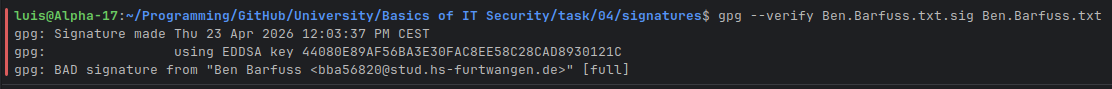
\includegraphics[width=\textwidth]{images/bad_signature}
	\caption{Signaturprüfung nach Manipulation der Datei}
\end{figure}

GPG meldet \textit{BAD signature}.
Das bedeutet, dass der Inhalt der Datei nach der Signierung verändert wurde.
Die Signatur stimmt nicht mehr mit dem aktuellen Dateiinhalt überein.
Dies zeigt, dass digitale Signaturen Manipulation zuverlässig erkennen.

\section*{h) Datei signieren und verschlüsseln}

Die Datei wurde mit dem eigenen Schlüssel signiert und für den Empfänger verschlüsselt:

\begin{lstlisting}[language=bash]
gpg --encrypt --sign --armor \
    -u lst48606@stud.hs-furtwangen.de \
    -r lst48606@stud.hs-furtwangen.de \
    LuisStaudt.txt
\end{lstlisting}

Als Empfänger wurde die eigene Adresse gewählt, um den Mechanismus zu demonstrieren.
Es entsteht die Datei \texttt{LuisStaudt.txt.asc}, die verschlüsselt und signiert ist.

\section*{i) Empfangene Datei entschlüsseln}

Die verschlüsselte Datei wurde mit folgendem Befehl entschlüsselt:

\begin{lstlisting}[language=bash]
gpg LuisStaudt.txt.asc
\end{lstlisting}

\begin{figure}[H]
	\centering
	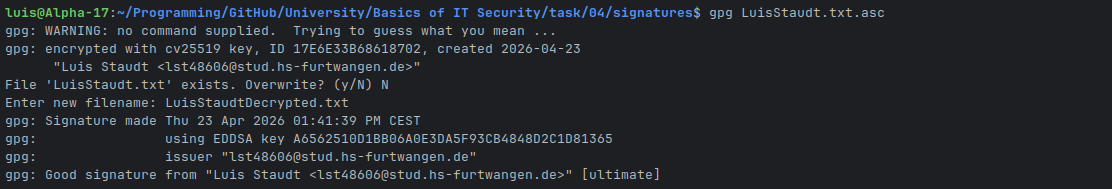
\includegraphics[width=\textwidth]{images/entschluesselung}
	\caption{Entschlüsselung und Signaturprüfung der verschlüsselten Datei}
\end{figure}

GPG meldet \textit{Good signature from \glqq Luis Staudt\grqq{} [ultimate]}.
Die Datei wurde mit dem privaten Schlüssel des Empfängers entschlüsselt und die
eingebettete Signatur erfolgreich geprüft.
Das zeigt, dass die Datei unverändert vom angegebenen Absender stammt.


\chapter*{Aufgabe 2: Aufbau einer Chain of Trust}

\section*{a) Signierten Schlüssel exportieren}

Nach dem gegenseitigen Signieren der Schlüssel wurde der öffentliche Schlüssel von Ben Barfuss
inklusive der eigenen Signatur exportiert:

\begin{lstlisting}[language=bash]
gpg --output Ben.Barfuss.signed.gpg --armor --export bba56820@stud.hs-furtwangen.de
\end{lstlisting}

Der Unterschied zum ursprünglich erhaltenen Schlüssel besteht darin, dass die exportierte Datei
nun zusätzlich die eigene Signatur enthält.
Andere Personen, die dieser Signatur vertrauen, können dadurch auch dem Schlüssel von Ben Barfuss
vertrauen, ohne ihn selbst verifiziert zu haben.

\section*{b) Schlüssel des Tutors}

Der öffentliche Schlüssel von \texttt{richard.zahoransky@hfu.eu} wird in der Praktikumsstunde
persönlich ausgetauscht und die Fingerprints gegenseitig geprüft.
Anschließend werden die Schlüssel mit \texttt{tsign} mit einer Trust-Tiefe größer 1 signiert,
damit das Vertrauen an andere Kommilitonen weitergegeben werden kann.

\section*{c) Signierten Zahoransky-Schlüssel importieren}

Der von einem Kommilitonen signierte öffentliche Schlüssel von richard.zahoransky wurde aus dem
Felix-Kurs heruntergeladen und importiert:

\begin{lstlisting}[language=bash]
gpg --import richard.zahoransky.signed.gpg
\end{lstlisting}

\section*{d) Signatur von ChainOfTrust.txt prüfen}

Die Datei \texttt{ChainOfTrust.txt} stammt von \texttt{richard.zahoransky@hfu.eu}.

GPG vertraut dieser Signatur, obwohl die Identität von richard.zahoransky nicht persönlich geprüft wurde,
weil ein Kommilitone dessen Schlüssel signiert hat, dem wiederum vertraut wird.
Durch die Trust-Tiefe größer 1 wird dieses Vertrauen weitergereicht.
GPG wertet das als ausreichenden Vertrauenspfad im Web of Trust.
Dies nennt sich \textit{Chain of Trust}: Vertrauen wird entlang einer Kette von Signaturen weitergegeben,
ohne dass jeder jeden persönlich kennen muss.


\chapter*{Aufgabe 3: Nutzen von GPG für den E-Mail-Versand}

\section*{a) Thunderbird einrichten}

Thunderbird wurde installiert und das Konto \texttt{lst48606@stud.hs-furtwangen.de} eingerichtet.

\section*{b) Privaten Schlüssel exportieren}

\begin{lstlisting}[language=bash]
gpg -o secret-key.gpg --export-secret-key
\end{lstlisting}

\section*{c) Öffentliche Schlüssel exportieren}

\begin{lstlisting}[language=bash]
gpg -o pub-keys.gpg --export
\end{lstlisting}

\section*{d–e) Schlüssel in Thunderbird importieren}

In den Kontoeinstellungen unter \textit{Ende-zu-Ende-Verschlüsselung} wurde der private Schlüssel
über \textit{Schlüssel hinzufügen} aus der Datei \texttt{secret-key.gpg} importiert.
Die öffentlichen Schlüssel der Kommilitonen wurden über die OpenPGP-Schlüsselverwaltung
unter \textit{Datei → Öffentliche Schlüssel importieren} hinzugefügt.

\section*{f) Signierte und verschlüsselte E-Mails}

Nach dem Import können E-Mails in Thunderbird signiert und verschlüsselt versendet werden.
Nicht einmal der Betreiber des E-Mail-Servers kann die verschlüsselten Inhalte lesen,
da nur der Empfänger mit seinem privaten Schlüssel entschlüsseln kann.

% ############################################################################
% CONTENT ENDS HERE
% ############################################################################

\end{document}
